\documentclass[a4paper, 12pt]{article}
\usepackage[utf8]{inputenc}
\usepackage[warn]{mathtext}
\usepackage[russian]{babel}
\usepackage[T2]{fontenc}
\usepackage[warn]{mathtext}
\usepackage[justification=centering]{caption}

\usepackage{graphicx}
\graphicspath{ {images/} }
\usepackage{tikz}
\usepackage{pgfplots}

\usepackage{amsmath}
\usepackage{floatflt}
\usepackage[left=20mm, top=20mm, right=20mm, bottom=20mm, footskip=10mm]{geometry}

\usepackage{multicol}
\usepackage{multirow}
\setlength{\columnsep}{2cm}

\usepackage{multicol}
\setlength{\columnsep}{2cm}
\usepackage{hyperref}
\usepackage{wrapfig}

\begin{document}
	
\begin{titlepage}
	\centering
	\vspace{5cm}
	{\scshape\LARGE Московский физико-технический институт \par}
	\vspace{4cm}
	{\scshape\Large Лабораторная работа 5.4.2 \par}
	\vspace{1cm}
	{\huge\bfseries Исследование энергетического спектра $\beta$-частиц и определение их максимальной энергии при помощи магнитного спектрометра \par}
	\vspace{1cm}
	\vfill
\begin{flushright}
	{\large выполнил студент 108 группы ФРКТ}\par
	\vspace{0.3cm}
	{\LARGE Трунов Владимир}
\end{flushright}
	

	\vfill

% Bottom of the page
	Долгопрудный, 2023  г.
\end{titlepage}

\paragraph*{Цель работы:} с помощью магнитного спектрометра исследовать энергетический спектр $\beta$-частиц при распаде ядер $^{137}$Cs и определить их максимальную энергию.

\section*{Теоретическая часть}
	
	Бета-распад - самопроизвольное превращение ядер, при котором их массовое число не изменяется, а заряд увеличивается или уменьшается на единицу.
	В данной работе:
	$$^A_Z X \to ^{\ \, A}_{Z+1} X + e^- + \widetilde{\nu} .$$
	
	Величина $W(p_e)$ является плотностью вероятности. Распределение электронов по энергии может быть вычислено теоретически. Для разрешенных переходов вероятность $\beta$-распада просто пропорциональна статистическому весу.
	\begin{equation*}
		\label{eq:W}
		W(p_e)dp_e \propto p_e^2(E_m-E_e)^2 dp_e.
	\end{equation*}
	Кинетическая энергия электрона и его импульс связаны друг с другом обычной формулой:
	\begin{equation*}
		E = \sqrt{(p_ec)^2+(m_ec^2)^2}-m_ec^2
	\end{equation*}
	Выражение (\ref{eq:W}) приводит к спектру, имеющему вид широкого колокола. Кривая плавно отходит от нуля и столь же плавно, по параболе, касается оси абсцисс в области максимального импульса электронов.
	
	Дочерние ядра, возникающие в результате $\beta$-распада, нередко оказываются возбужденными. Возбужденные ядра отдают свою энергию либо излучая $\gamma$-квант, либо передавая избыток энергии одному из электронов внутренних оболочек атома. Излучаемые в таком процессе электроны имеют строго определенную энергию и называются \textit{конверсионными}.
	
	Конверсия чаще всего происходит на оболочках K и L. Ширина конверсионной линии является чисто аппаратурной -- по ней можно оценить разрешающую силу спектрометра.
	
\section*{Экспериментальная установка}
	Блок-схема установки для изучения $\beta$-спектров изображена на рис. \ref{pic1}. Радиоактивный источник $^{137}$Cs помещен внутрь откачанной трубы. Электроны, сфокусированные магнитной линзой, попадают в счетчик. В газоразрядном счетчике они инициируют газовый разряд и тем самым приводят к появлению электрических импульсов на электродах, которые затем регистрируются счетным прибором.
    
    \begin{figure}[h]
    \centering
    \begin{minipage}{.5\textwidth}
      \centering
      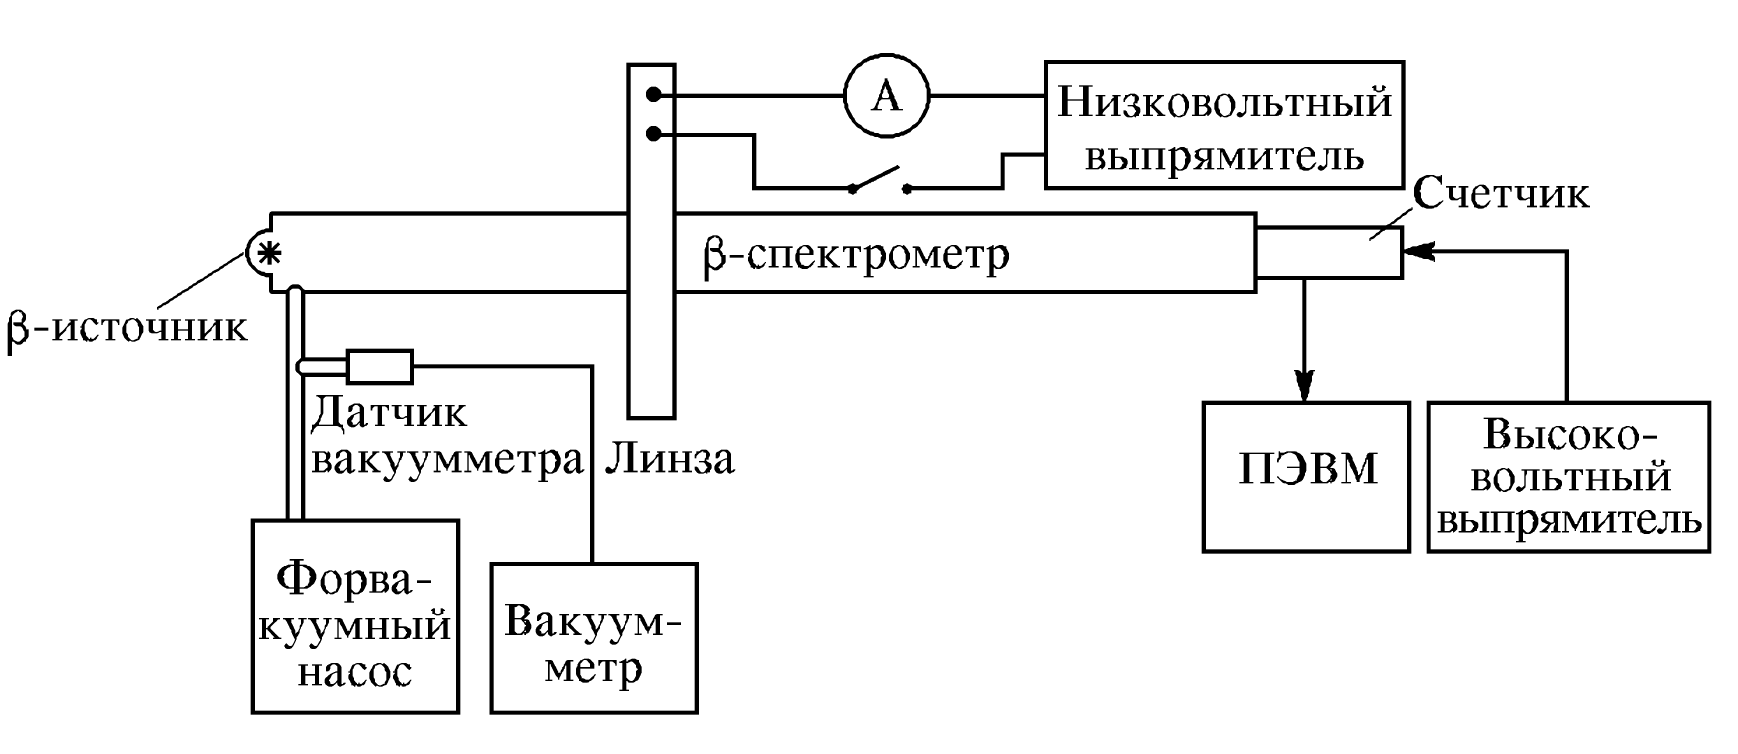
\includegraphics[width=\linewidth]{scheme.png}
      \captionof{figure}{Схема установки}
      \label{fig:test1}
    \end{minipage}%
    \begin{minipage}{.5\textwidth}
      \centering
      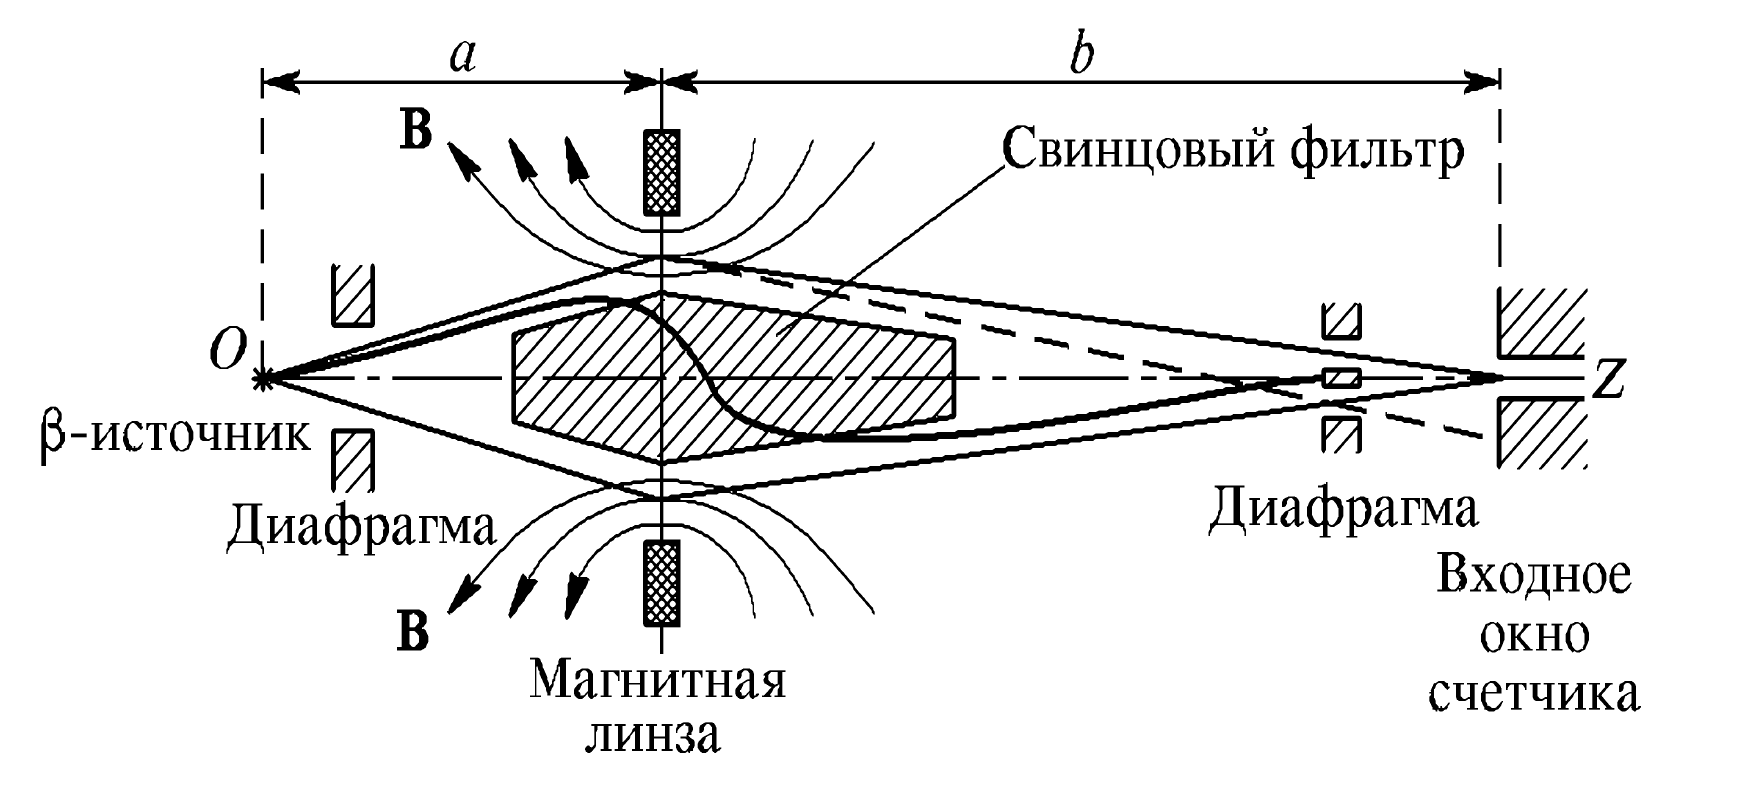
\includegraphics[width=\linewidth]{equip.png}
      \captionof{figure}{Принцип работы}
      \label{fig:test2}
    \end{minipage}
    \end{figure}
	
	Энергию $\beta$-частиц определяют с помощью $\beta$-спектрометров (рис.~\ref{pic2}). В работе используется магнитный спектрометр с <<короткой линзой>>. Отметим, что в течение всего опыта геометрия прибора остается неизменной, поэтому импульс сфокусированных электронов пропорционален величине тока:
	\begin{equation}
		\label{eq:pkI}
		\tag{$\star$}
		p_e = kI.
	\end{equation}

	Cвязь между числом частиц, регистрируемых установкой, и функцией $W(p_e)$ выражается формулой:
	\begin{equation*}
		N(p_e) \propto W(p_e)p_e,
	\end{equation*}
	откуда
	\begin{equation}
		\label{eq:fermi}
		\tag{$\star \star$}
		\frac{\sqrt{N}}{p_e^{3/2}} \propto E_m - E
	\end{equation}
	
	
	\section*{Экспериментальные данные}
		
		\begin{table}[h]
		\centering
		\caption{Результаты измерений}
		\label{table:data}
        \begin{tabular}{|l|l|l|l|l|l|}
    \hline
        I, $\text{А}$ & N, $\frac{1}{\text{c}}$   & N - ${N_\text{ф}}$, $\frac{1}{\text{c}}$ & p, $\frac{\text{кэВ}}{\text{с}}$  & T, $\text{кэВ}$ & $\frac{\sqrt{N(p)}}{p^{\frac{3}{2}}}$, $\frac{\text{c}}{\text{м}^{\frac{3}{2}}}$\\ \hline
        0,00 & 0,70 & -0,01 & 0,00 & 0,00 & 0,00 \\ \hline
        0,20 & 8,77 & -0,02 & 49,40 & 2,40 & 0,00 \\ \hline
        0,40 & 1,08 & 0,30 & 98,80 & 9,50 & 557,26 \\ \hline
        0,60 & 0,85 & 0,07 & 148,20 & 21,10 & 146,33 \\ \hline
        0,80 & 0,97 & 0,20 & 197,60 & 36,90 & 156,76 \\ \hline
        1,00 & 1,58 & 0,80 & 247,00 & 56,60 & 230,27 \\ \hline
        1,20 & 1,66 & 0,88 & 296,50 & 79,80 & 183,73 \\ \hline
        1,40 & 2,90 & 2,12 & 345,90 & 186,00 & 226,32 \\ \hline
        1,68 & 3,25 & 2,47 & 395,30 & 135,00 & 199,95 \\ \hline
        1,80 & 4,04 & 3,26 & 444,70 & 166,40 & 192,51 \\ \hline
        2,00 & 3,88 & 3,90 & 494,10 & 199,80 & 160,28 \\ \hline
        2,20 & 5,04 & 4,26 & 543,50 & 235,00 & 162,87 \\ \hline
        2,40 & 4,84 & 4,06 & 592,90 & 271,70 & 139,54 \\ \hline
        2,60 & 4,66 & 3,88 & 642,30 & 309,80 & 120,98 \\ \hline
        2,80 & 4,18 & 3,40 & 691,70 & 349,00 & 101,33 \\ \hline
        3,00 & 3,75 & 2,97 & 741,10 & 389,20 & 85,40 \\ \hline
        3,20 & 2,98 & 2,20 & 790,50 & 430,30 & 66,72 \\ \hline
        3,40 & 1,67 & 0,89 & 840,80 & 472,20 & 38,74 \\ \hline
        3,60 & 1,26 & 0,48 & 889,40 & 514,70 & 26,11 \\ \hline
        3,80 & 1,62 & 0,84 & 938,80 & 557,80 & 31,85 \\ \hline
        4,00 & 5,03 & 4,25 & 988,20 & 601,50 & 66,35 \\ \hline
        4,10 & 7,46 & 6,68 & 1012,90 & 623,50 & 80,16 \\ \hline
        4,20 & 5,48 & 4,70 & 1837,60 & 645,60 & 64,85 \\ \hline
        4,30 & 5,19 & 4,41 & 1862,30 & 667,80 & 60,64 \\ \hline
        4,40 & 2,31 & 1,53 & 1887,00 & 690,10 & 34,51 \\ \hline
        4,60 & 8,59 & -0,20 & 1136,40 & 735,00 & 0,00 \\ \hline
        4,80 & 0,61 & -0,17 & 1185,80 & 780,20 & 0,00 \\ \hline
        5,00 & 0,42 & -0,36 & 1235,20 & 825,70 & 0,00 \\ \hline
    \end{tabular}
        \end{table}
	

	\section*{Обработка результатов}
		По результатам измерений (табл.~\ref{table:data}) построим график cпектра $\beta$-распада атома $^{137}$Cs и откалибруем его. Для этого пересчитаем значения силы тока в импульс по формуле (\ref{eq:pkI}). Коэффициент $k$ определим по известной конверсионной линии:
			$$624 \ \text{кэВ} = kcI_0,$$
		где $c$ -- скорость света, $I_0 = 4,1$ А -- сила тока, при которой наблюдается конверсионный пик.

            \begin{center}
            $k$ = 154,6 $\frac{\text{кэВ}}{{\text{с}} \cdot {\text{А}}}$
            \end{center}
  
	\begin{figure}[h]
		\centering
            \includegraphics[width=10cm]{N-Nф.png}
            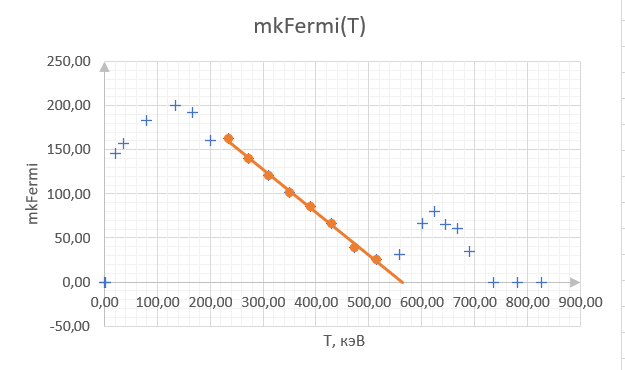
\includegraphics[width=12cm]{mkFermi.png}
            \caption{$\text{N(J)}$ и график Ферми}
        \end{figure}

		Определим максимальную энергию $\beta$-спектра. Анализ спектральной картины $\text{N(J)}$ в таком случае даст достаточно грубый результат, так как нам придётся ограничиться исследованием точек у самой верхней границы спектра. Эти точки измерены с наименьшей статистической точностью. Однако мы можем уменьшить ошибку определения максимальной энергии посредством процедуры Ферми-Кюри. Для этого мы отложим по оси ординат величину $\sqrt{N}/p^{3/2}$, а по оси абсцисс энергию $\beta$-частиц (с учётом того, что энергия электронов внутренней конверсии $^{137}$Cs равна 634 кэВ). В таком случае мы задействуем большинство экспериментальных точек, и прежде всего точки середины $\beta$-спектра, которые измерены с наилучшей точностью.
		
		Получим максимальную энергию частиц:
		
		\[E_{m} = 560\pm 7 \text{кэВ}\]
		
		
	
        \begin{figure}[h]
		\centering
            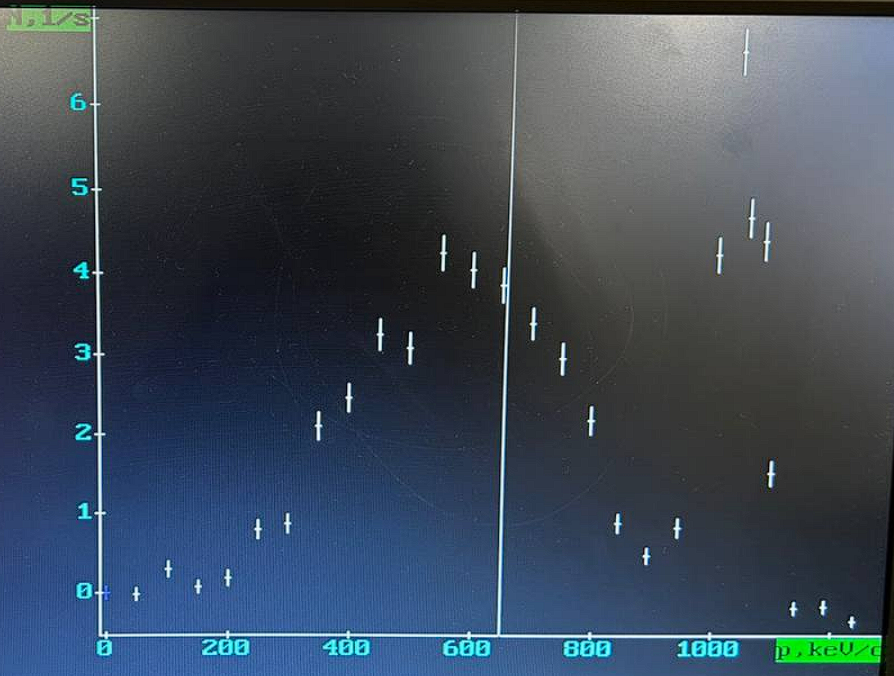
\includegraphics[width=10cm]{p.png}
            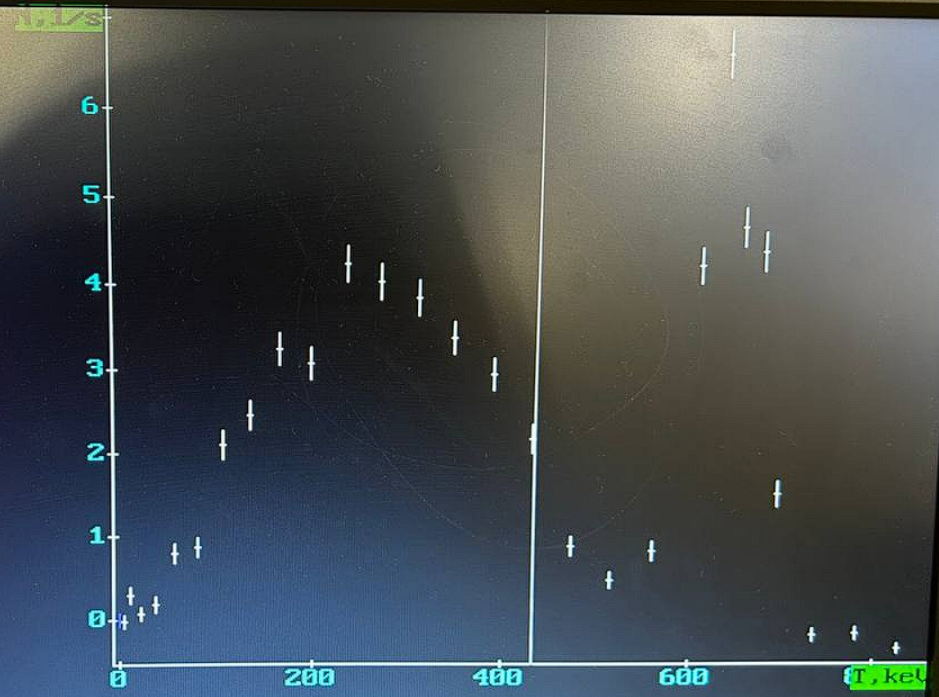
\includegraphics[width=10cm]{T.png}
            \caption{$\text{N(p)}$ и $\text{N(T)}$}
        \end{figure}

\end{document}